\chapter{MACROECONOMICS}
\begin{chapquote}{Roberto Bordin}
``La figa e' l'oppio dei popoli.''
\end{chapquote}

This is an additional chapter and can be useful to have a better understanding of what is going on in the world. The following sections are inspired by the online course available at \url{https://www.khanacademy.org/economics-finance-domain/macroeconomics}. It will be expanded in the future with more sections to cover more topics (Austrian economics for example).

\section{Circular flow of income and expenditures}
Imagine we have a country with only a firm and one family that owns the firm. The firm needs some factors of production building, land and labor to create products. This will produce some profit for the company. In this scenario, the family is buying from the firm, the firm is providing products to the family. On the other side, the family is providing the production factors to the firm and the firm is giving money to the family in form of wages, profit and rent for the other production factors. In this example, we have a family with the total expenditures, the firm with the total revenues, but also again the family with the total income. Expenditures and revenues are the same in this case, but all the revenues go to the family for paying the production factors and profit. Even if a bit artificial, this can be extended to the circular flow of money in a country with multiple firms and households. The gross domestic product (GDP) can be the total expenditures of the family, the total revenue of the firm or the total income of again the family, because they are all the same.

More formally, the GDP is the market value of all final products and services produced within a country in a given period. We do not count though illegal activity, or labor like a mother babysitting her own child. If the production of a good lasts longer than the period considered for computing the GDP, then the market value of the intermediate good (not finished yet) is considered. The following period will then consider the market value of the final good (assuming it is finished in this second period) minus the market value at the beginning of the period. Moreover, the goods taken into account are the ones produced within a country, regardless of the nationality of the producer. The gross national product (GNP) does instead take into account the nationality of the firm and not where the firm is based.

\subsection{How well GDP measures the well-being of society}
GDP is an indicator of a society’s standard of living, but it is only a rough indicator. 

GDP does not account for leisure time. The US GDP per capita is larger than the GDP per capita of Germany, but does this prove that the standard of living in the United States is higher? Not necessarily since it is also true that the average US worker works several hundred hours more per year more than the average German worker. The calculation of GDP does not take German workers extra weeks of vacation into account.

GDP includes what is spent on environmental protection, healthcare, and education, but it does not include actual levels of environmental cleanliness, health, and learning. GDP includes the cost of buying pollution-control equipment, but it does not address whether the air and water are actually cleaner or dirtier. GDP includes spending on medical care, but it does not address whether life expectancy or infant mortality have risen or fallen. Similarly, GDP counts spending on education, but it does not address directly how much of the population can read, write, or do basic mathematics.
GDP includes production that is exchanged in the market, but it does not cover production that is not exchanged in the market. 
GDP has nothing to say about the level of inequality in society. GDP per capita is only an average. When GDP per capita rises by 5\%, it could mean that GDP for everyone in the society has risen by 5\% or that the GDP of some groups has risen by more while the GDP of others has risen by less—or even declined.

GDP also has nothing in particular to say about the amount of variety available. If a family buys 100 loaves of bread in a year, GDP does not care whether they are all white bread or whether the family can choose from wheat, rye, pumpernickel, and many others—GDP just looks at whether the total amount spent on bread is the same.
Likewise, GDP has nothing much to say about which technology and products are available. The standard of living in, for example, 1950 or 1900 was not affected only by how much money people had—it was also affected by what they could buy. No matter how much money you had in 1950, you could not buy an iPhone or a personal computer.

In certain cases, it is not clear that a rise in GDP is even a good thing. If a city is wrecked by a hurricane and then experiences a surge of rebuilding construction activity, it would be peculiar to claim that the hurricane was therefore economically beneficial. If people are led by a rising fear of crime to pay for installation of bars and burglar alarms on all their windows, it is hard to believe that this increase in GDP has made them better off. In that same vein, some people would argue that sales of certain goods, like pornography or extremely violent movies, do not represent a gain to society’s standard of living.

The fact that GDP per capita does not fully capture the broader idea of standard of living has led to a concern that the increases in GDP over time are illusory. It is theoretically possible that while GDP is rising, the standard of living could be falling if human health, environmental cleanliness, and other factors that are not included in GDP are worsening. Fortunately, this fear appears to be overstated.
In some ways, the rise in GDP actually understates the actual rise in the standard of living. For example, the typical workweek for a US worker has fallen over the last century from about 60 hours per week to less than 40 hours per week. Life expectancy and health have risen dramatically, and so has the average level of education.
Since 1970, the air and water in the United States have generally been getting cleaner. New technologies have been developed for entertainment, travel, information, and health. A much wider variety of basic products like food and clothing is available today than several decades ago. GDP does not capture leisure, health, a cleaner environment, the possibilities created by new technology, or an increase in variety.
On the other side, rates of crime, levels of traffic congestion, and inequality of incomes are higher in the United States now than they were in the 1960s. Moreover, a substantial number of services that used to be provided, primarily by women, in the nonmarket economy are now part of the market economy that is counted by GDP. By ignoring these factors, GDP would tend to overstate the true rise in the standard of living.

A high level of GDP should not be the only goal of macroeconomic policy—or broader government policy. But, even though GDP does not measure the broader standard of living with any precision, it does measure production well, and it does indicate when a country is materially better or worse off in terms of jobs and incomes. In most countries, a significantly higher GDP per capita occurs hand in hand with other improvements in everyday life along many dimensions, like education, health, and environmental protection.

\subsection{Investment and consumption}
In everyday life, an investment is something that will give you a future gain like having a house, having a bond, studying, while consumption is when you use money to use up something and should make your life better in the short term.

In economy instead, investments are the creation of capital equipment, inventories for firms and construction of new houses while consumption is any spending on new final goods or services by households, except for new homes

For example, buying a car to go to work can be seen as an investment from the first perspective, but as a consumption from the second perspective.

\subsection{Expenditure view and components of GDP}
The GDP is made of the expenditures of the firms and of the households and of the government plus the exports minus the imports. To differentiate the expenditures between investment and consumption we can say that $Y = I + C + G + NX$, where $Y$ is the GDP and the other terms are the investments (both from firms and households), the consumption, the expenditures of the government and the net export. If an American firm is investing money on a foreign production factor, it means the investment value increases, but the net export decreases correspondingly and the total GPD does not change.

It's important to remember that a significant portion of government budgets are transfer payments—like unemployment benefits, veteran’s benefits, and Social Security payments to retirees—that are excluded from GDP because the government does not receive a new good or service in return or exchange. The only part of government spending counted in demand is government purchases of goods or services produced in the economy—for example, a new fighter jet purchased for the Air Force (federal government spending), construction of a new highway (state government spending), or building of a new school.

Since every market transaction must have both a buyer and a seller, GDP must be the same whether measured by what is demanded or by what is produced.
Everything that is purchased must be produced first. Instead of trying to think about every single product produced, let's break out five categories: durable goods, non-durable goods, services, structures, and change in inventories. 

You can see what percentage of the GDP each of these components contributes in the table and pie chart below.

\begin{figure}
\makebox[\textwidth][c]{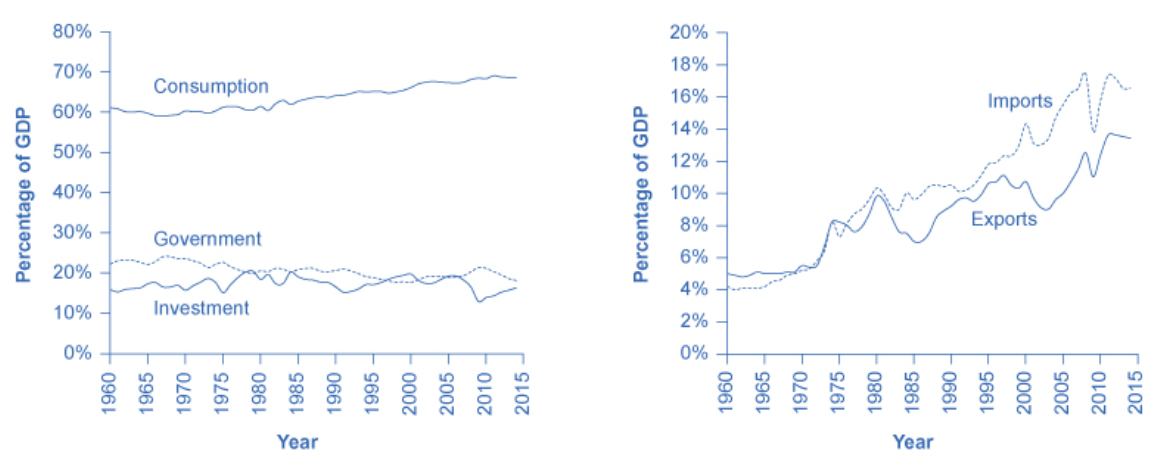
\includegraphics[width=1.1\textwidth]{images/USA_GDP.png}}
    \caption{GDP of the USA.}
    \label{fig:usa_gdp1}
\end{figure}

\begin{figure}
\makebox[\textwidth][c]{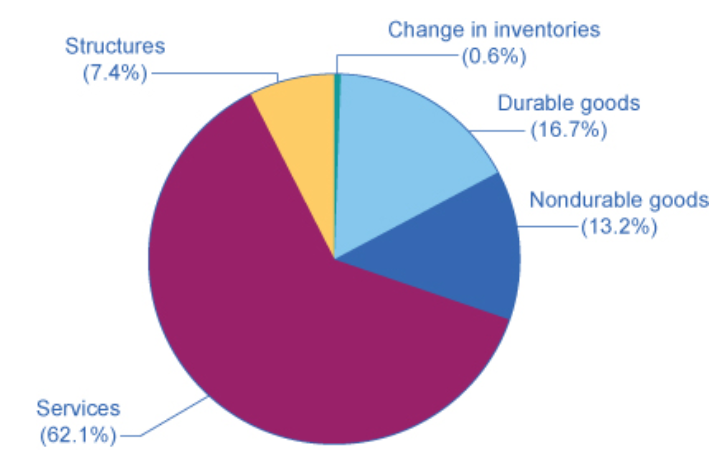
\includegraphics[width=1.1\textwidth]{images/USA_GDP_pie.png}}
    \caption{GDP of the USA.}
    \label{fig:usa_gdp_pie}
\end{figure}


The category of structures includes everything from homes to office buildings, shopping malls, and factories.
Inventories is a small category that refers to the goods that have been produced by one business but have not yet been sold to consumers and are still sitting in warehouses and on shelves.

The entire underground economy of services paid “under the table” and illegal sales should be counted—but is not—because it is impossible to track these sales. In a recent study by Friedrich Schneider of shadow economies, the underground economy in the United States was estimated to be 6.6\% of GDP, or close to \$2 trillion dollars in 2013 alone.

\subsection{Other ways to measure the economy}
Gross national product, or GNP, includes what is produced domestically and what is produced by domestic labor and business abroad in a year.
National income includes all income earned: wages, profits, rent, and profit income.
Net national product, or NNP, is GNP minus depreciation.
Depreciation is the process by which capital ages over time and therefore loses its value.

\subsection{Nominal and real GDP}
Let's say we have a country producing only oranges and at the end of year 1 we have a GDP equal to $Y_1 = N_1 p_1$, where $N_1$ is the amount of oranges produced in year 1 and $p_1$ is the price of one orange in year 1. At the end of year 2 we have instead $Y_2 = N_2 p_2$ and we can measure the growth of the country in this way: $G = Y_2 - Y_1$. Here, we are using the nominal GDP. If $G$ is positive, we might think that the economy is now larger than before, but did the country actually produced more goods than the previous year? Or in other terms, what is the GDP of year 2 in year 1's prices? This is the real GPD of year 2 and is equal to $Y_2' = N_2 p_1$.

\subsection{GDP deflator}
The GDP deflator is a measure of price inflation/deflation with respect to a specific base year; the GDP deflator of the base year itself is equal to 100.
\begin{equation}
GDP deflator = \dfrac{Nominal GDP}{Real GDP} 100
\end{equation}
The higher the GDP deflator, the lower the real GDP will be compared to the nominal GDP.

\subsection{Income and inequality}
\begin{figure}
\makebox[\textwidth][c]{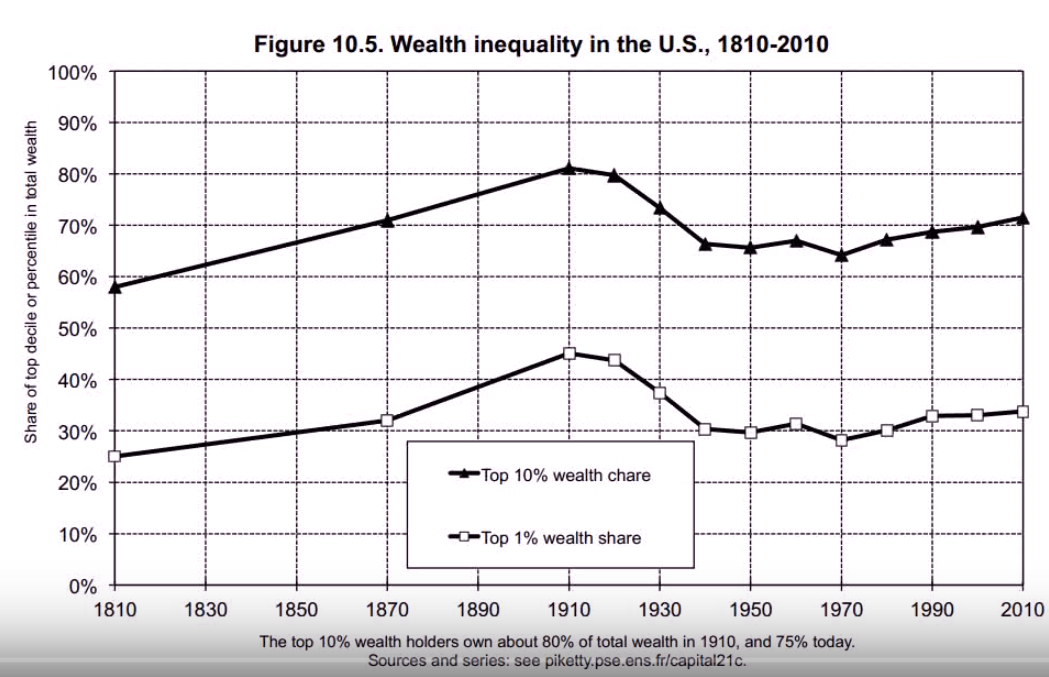
\includegraphics[width=1.1\textwidth]{images/piketty.png}}
    \caption{From Capital in the twenty-first century by Thomas Piketty.}
    \label{fig:piketty}
\end{figure}

Wealth is the total value of the assets owned by a person, which is different from its income. Thomas Piketty draws two possible theories of why we have income inequality. One is driven by labor where we have a mix of two possible reasons: the market recognizes the importance of top managers that are able to make big profits for the company, but also because these top managers are also self-regulating their income. The other theory is based on return on capital (ROC) and its relationship with the growth of the economy. If a person has a big amount of money inherited and she invest it, the ROC might be large enough to live without working. If the ROC is larger than the growth of the economy, the income inequality will grow. An example is the following. Alice gets \$100k in after-tax income, she spends \$80k and saves 20\% of her income, while Bob gets \$1M in after-tax income, spends \$400k and saves 60\%. Bob is getting richer because he's saving more, because it's easier to save money. As your income becomes smaller, it is more difficult to save. Because the saving rates generally goes up, more people will be in the situation of $r > g$, meaning that the ROC is greater than the growth of the economy. 

\begin{figure}
\makebox[\textwidth][c]{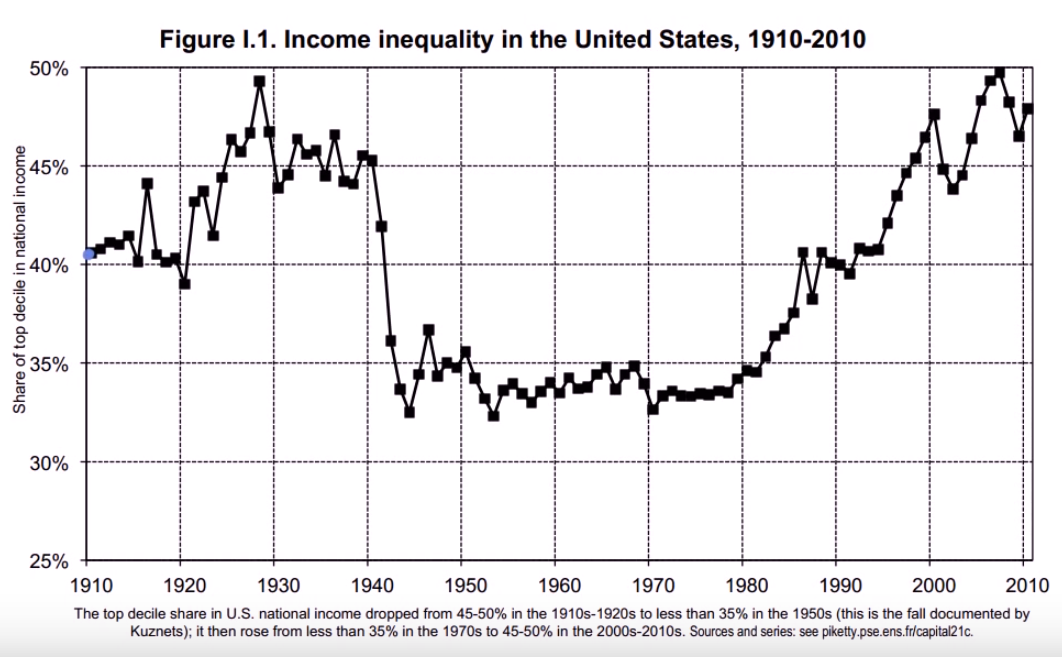
\includegraphics[width=1.1\textwidth]{images/income_ineq.png}}
    \caption{From Capital in the twenty-first century by Thomas Piketty.}
    \label{fig:income_ineq}
\end{figure}

A question to ask is: Is inequality always bad? There might be an example in which the answer is no.
Let's imagine a country in which the GDP is equal to 100 (whatever the currency) and the top 10\% of the people owns a third of the GPD. This means that the bottom 90\% of the population owns 67\% of the GPD, which means that each person in the bottom 90\% owns 0.741\% of the GPD, hence 0.741 (whatever the currency), and each person in the top 10\% holds 3.333\% of the GPD, hence 3.333 (whatever the currency). Now imagine a situation in which after one year, the GPD grew 10\%. This happens thanks to capital markets, which also bring more inequality. Let's also imagine that the top 10\% of the people holds now 35\% of the GPD which means two things: higher inequality and each of them has 3.5\% of the GDP, or 3.85 (because the GDP is now 110). But it also means that the bottom 90\% now has 65\% of the GDP, or 71.5 (whatever the currency), which means 0.794 for each person, larger than 0.741 of the previous year. So, in this example, we have growth, more inequality, but all the population got better. In general, if economic growth is enough, there will be a bigger pie for everyone. 

If you had to choose between a static economy and a personal income of X, or a growing economy and a personal income of X plus something, what would you choose? Remember that in the second case, someone will get a larger share of the growth than you, but still you will improve the quality of your life.

One force that was able to reduce inequality and led to more development in Asia after 1950 is education. In the gilded age (end of 19th century) there was no need of highly-skilled labor and capital had lot of importance in the production line. Now instead, especially with technology, more and more focus is put on educated labor (e.g., software and services).

Why does the value of private capital grow faster than national income? Imagine today you buy an asset (capital) with a value $V$ and it will give you a ROC of $r$, so the income is $rV$. In few months, for some reason, the same asset will give an income of $2rV$, but because there is a lot of people demanding this asset now, its value is $2V$, hence its ROC is still $r$. This means that people are still willing to have that asset with the same ROC, but the value of the capital and the income it generates has increased. But it could also happen the opposite, where the income decreases, then the value decreases and the ROC remains the same. Another possible scenario is when there is more money and less profitable businesses. In this case, people will be willing to have a lower ROC, so if the income is still $rV$, but $r$ is lower, than $V$ must increase.

Today:
\begin{itemize}
    \item V = 100
    \item I = 10
    \item r = 10\%
\end{itemize}
Tomorrow with more profitable businesses (in terms of income), but more people investing:
\begin{itemize}
    \item V = 200
    \item I = 20
    \item r = 10\%
\end{itemize}
Tomorrow with less profitable businesses (in terms of income), and less people investing:
\begin{itemize}
    \item V = 50
    \item I = 5
    \item r = 10\%
\end{itemize}
Tomorrow with less profitable businesses (in terms of ROC), and more people investing:
\begin{itemize}
    \item V = 200
    \item I = 10
    \item r = 5\%
\end{itemize}
Tomorrow with less profitable businesses (in terms of ROC), and less people investing:
\begin{itemize}
    \item V = 50
    \item I = 2.5
    \item r = 5\%
\end{itemize}

\subsection{Bond prices and interest rates}
If in this moment the interest rates increase, the prices of the bonds available in the market few seconds ago will decrease.

Let's illustrate this with a \$100,000 bond having a stated interest rate of 9\% and having a remaining life of 5 years. This bond will pay \$4,500 at the end of each of the 10 remaining semiannual periods plus \$100,000 at the end of the bond's life. If an investor's goal is to earn 9\%, the investor will pay \$100,000 for the bond. However, if the market interest rates increase to 10\% the investor will now be able to earn \$5,000 semiannually on a \$100,000 investment. Obviously, the 9\% bond paying only \$4,500 semiannually will no longer be salable for \$100,000.

For an investor to buy the 9\% bond in a 10\% market, the bond's price will have to drop to an amount that will yield a 10\% return over the bond's remaining life. Using our example, the investor will earn 10\% only if the 9\% bond can be purchased for approximately \$96,000. The cash return of \$4,500 every six months for five years on the \$96,000 investment plus the gain of \$4,000 (\$100,000 in 5 years versus the investment of \$96,000) will result in the required return of 10\%.


\section{Inflation: measuring the cost of living}

\subsection{Unintended redistributions of purchasing power and inflation}
Inflation can cause redistributions of purchasing power that hurt some and help others. People who are hurt by inflation include those who are holding a lot of cash, whether it is in a safe deposit box or in a cardboard box under the bed. When inflation happens, the buying power of cash is diminished. But cash is only an example of a more general problem: anyone who has financial assets invested in a way that the nominal return does not keep up with inflation will tend to suffer from inflation. For example, if a person has money in a bank account that pays 4\% interest, but inflation rises to 5\%, then the real rate of return for the money invested in that bank account is negative 1\%.

The US income tax is charged on the nominal interest received in dollar terms, without an adjustment for inflation. So, a person who invests \$10,000 and receives a 5\% nominal rate of interest is taxed on the \$500 received—no matter whether the inflation rate is 0\%, 5\%, or 10\%. If inflation is 0\%, then the real interest rate is 5\% and all \$500 is a gain in buying power. But if inflation is 5\%, then the real interest rate is zero and the person had no real gain—but they owe income tax on the nominal gain anyway. If inflation is 10\%, then the real interest rate is negative 5\%, and the person is actually falling behind in buying power. But, they would still owe taxes on the \$500 in nominal gains.

Inflation can cause unintended redistributions for wage earners, too. Wages do typically creep up with inflation over time—eventually. However, increases in wages may lag behind inflation for a year or two since wage adjustments are often somewhat sticky and occur only once or twice a year. Also, the extent to which wages keep up with inflation creates insecurity for workers and may involve painful, prolonged conflicts between employers and employees. 
Ordinary people can sometimes benefit from the unintended redistributions of inflation as well. Consider someone who borrows \$10,000 to buy a car at a fixed interest rate of 9\%. If inflation is 3\% at the time the loan is made, then the loan must be repaid at a real interest rate of 6\%. But if inflation rises to 9\%, then the real interest rate on the loan is zero. In this case, the borrower’s benefit from inflation is the lender’s loss. A borrower paying a fixed interest rate who benefits from inflation is just the flip side of an investor receiving a fixed interest rate who suffers from inflation. The lesson is that when interest rates are fixed, rises in the rate of inflation tend to penalize suppliers of financial capital, who end up being repaid in dollars that are worth less because of inflation. At the same time, demanders of financial capital end up better off because they can repay their loans in dollars that are worth less than originally expected.

When inflation causes a retiree who built up a pension or invested at a fixed interest rate to suffer while someone who borrowed at a fixed interest rate benefits from inflation, it is hard to believe that this outcome was deserved in any way. 

A firm can make money from inflation—for example, by paying bills and wages as late as possible so that it can pay in inflated dollars, while collecting revenues as soon as possible. A firm can also suffer losses from inflation, as in the case of a retail business that gets stuck holding too much cash only to see the value of that cash eroded by inflation. But when a business spends its time focusing on how to profit by inflation, or at least how to avoid suffering from it, an inevitable trade-off strikes: less time is spent on improving products and services or on figuring out how to make existing products and services more cheaply. An economy with high inflation rewards businesses that have found clever ways of profiting from inflation, which are not necessarily the businesses that excel at productivity, innovation, or quality of service.

Traditionally, government bonds have paid a fixed rate of interest. This policy gave a government that had borrowed an incentive to encourage inflation because it could then repay its past borrowing in inflated dollars at a lower real interest rate. But indexed bonds promise to pay a certain real rate of interest above whatever inflation rate occurs. In the case of a retiree trying to plan for the long term and worried about the risk of inflation, for example, indexed bonds that guarantee a rate of return higher than inflation—no matter the level of inflation—can be a very comforting investment.

\subsection{Phillips curve}

Irving Fisher, and later William Phillips, showed that there is an inverse relationship between unemployment and inflation: High inflation means higher prices due to higher demand, due to higher wages, due to more leverage for workers, due to lower unemployment. Two exceptions must be considered. The first happened in 1970, when the oil supply suddenly decreased and drove the prices up, but it was not due to higher wages, so there chain presented above was broken. The second happened with the technological revolution where more demand did not cause lower unemployment because of higher production and production efficiency.

\section{Aggregate demand and aggregate supply}
\subsection{Aggregate demand}
Aggregate demand is the amount of total spending on domestic goods and services in an economy.

In microeconomics, production and prices have a negative correlation: all else being equal, more production means lower price. Some economists claim that this is true also in macroeconomics and the aggregate demand curve is similar to the downward-sloping demand curve. There are three theories supporting this. If one day, prices decrease within a country, people will have more buying power, so they could buy more or save more. In the first case, they directly stimulate more production, while in the second case they put more money in the banks, which will be able to lower interest rates and make more investments and then the general production of the country increases. The third case is still based on the fact that interest rates are lower and investors would convert money into another currency with higher interest rates, making the own country's currency weaker, stimulating export, hence more production (GDP).

If the GPD is the sum of consumption, investments, government spending and net export, then any increment in one of these factors will move the curve right.

\subsection{Aggregate supply}
Aggregate supply is the total quantity of output firms will produce and sell—in other words, the real GDP. 

In the long term, which means a period in which fixed contracts expire, real GDP does not change with the prices. It increases or decreases though thanks to other factors: increase in population, higher employment, technological 
improvement, wars, discovery of new resources. In the long run, the price doesn't matter because any increases or decreases in price will be cancelled out by decreases or increases in costs (wages, input costs, etc.). If prices double, so do wages, so people have no additional spending power. Firms will produce the same and households will buy the same.

Over time, productivity grows so that the same quantity of labor can produce more output. Historically, the real growth in GDP per capita in an advanced economy like the United States has averaged about 2\% to 3\% per year, but productivity growth has been faster during certain extended periods.

In the short term instead, we have an upward-sloping aggregate supply curve, because when the price level for outputs increases while the price level of inputs remains fixed, the opportunity for additional profits encourages more production.

Demand curves for individual goods or services slope down primarily because of the existence of substitute goods, not the wealth effects, interest rate, and foreign price effects associated with aggregate demand curves.

\subsection{Demand-pull and cost-push inflation}
In the '60 the US president Johnson kept spending and investing at an excessive level. This put more money into people's pockets and the real GDP increased, shifting the aggregate demand curve to the right. The equilibrium between aggregate demand and aggregate supply on the short was at a higher level of prices and of real GDP (beyond the natural level). On the long term though, the aggregate demand must meet the aggregate supply on the long run, so the prices are higher if aggregate demand does not go back to its previous level.

In the 1973 we had the oil embargo in the US that led to higher prices in general, without any increment in the real GDP. This led to shift the short term aggregate supply curve to the left, because it was more expensive to produce goods. This is stagflation.

\subsection{Monetary and fiscal policy}
How is the demand and supply for the money market? On the x-axis we have the money supply (how much money are available to be borrowed/lent), on the y-axis we have the price of borrowing, namely interest rates. The demand curve is decreasing with supply because the cheaper the cost of money, the higher the number of people willing to borrow for their projects. Very few projects have high returns and many projects have low returns. The aggregate supply instead is increasing: the higher the interest rate, the better for the supplier (lender), the higher the number of lenders. 

When the central bank lends money, it is shifting the supply curve to the right, making it easier for people to borrow money and start businesses and to spend money, leading to an increase of aggregate demand. This is known as monetary policy.

Fiscal policy is instead used by the government to stimulate or slow down demand leveraging on taxes and debt. This policy has usually a more direct effect.

\subsection{Keynesian economics}
The classical model for aggregate demand and aggregate supply in the long run is a vertical line for LRAS and a downward-sloping AD. The only way to increase the output of the country is by making it more productive through investments in technology or increase population for example, to shift the LRAS to the left. Just flooding the economy with newly printed money will increase the demand, but in the long run aggregate supply will not change, only prices and inflation will.

One reasoning that makes sense is the following: If the economy is working at full capacity, people will be very busy to work, they would make good money and don't need to work extra time to survive. If they are asked to do extra work, they would ask for a pay raise and prices would go up. On the other hand, if unemployment is high, people will not ask for higher salaries and in the short run, they will be willing to get the same salary regardless of working time. If a factory is running at \%30 capacity and people wants to buy more from me, I'm not going to raise prices because I still need to attract clients. In other words, at low capacity and in the short run prices are sticky compared to production.

In the '30, during the Great Depression factories and people were available to work, but aggregate demand decreased significantly and quickly. The economy was producing below its capacity. At this point, Keynes believed that the SRAS is a horizontal line. In this case the only way to increase GPD is to increase the aggregate demand, through monetary policy or fiscal policy.

In conclusion, the most appropriate model is a mix of classical and Keynesian economics. At low real GDP levels, prices do not change with production and the government should increase the aggregate demand, while at high real GDP levels production does not change with prices and if the government wants to further increase production, it should increase population of production efficiency.

The risk associated to Keynesian politics is that once the government intervenes through fiscal policy (taxes or spending), it becomes difficult and unpopular to stop these stimuli and this might lead to a overheated economy and a growing inflation without a corresponding increase in real GDP because everything is spent on consumption and nothing is saved for technological improvements\footnote{I think the key part here is how the government is using the extra money obtained through monetary or fiscal policy. With Keynesian politics, it should use it to increase aggregate demand, ignoring investments to increase the aggregate supply. What if instead some part if it is used also to increase the aggregate supply?}.

\begin{figure}
\makebox[\textwidth][c]{
    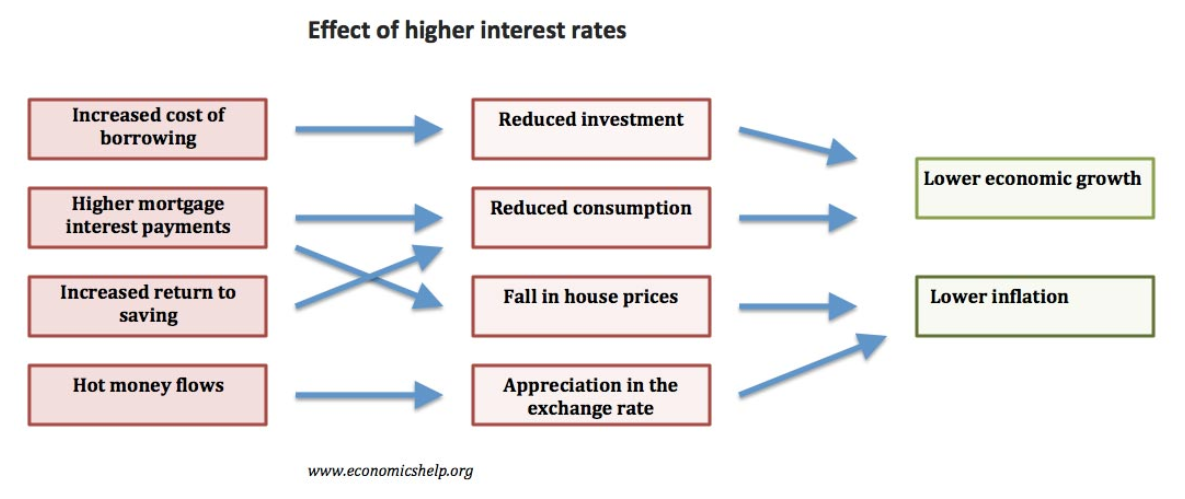
\includegraphics[width=1.1\textwidth]{images/high_rates.png}
}
    \caption{Why should a central bank make borrowing more difficult?}
    \label{fig:high_rates}
\end{figure}

The Central Bank usually increase interest rates when inflation is predicted to rise above their inflation target. They increase the cost of borrowing, reduce disposable income and therefore limit the growth in consumer spending. Higher interest rates tend to reduce the rate of economic growth and inflationary pressures. Higher interest rates make it more attractive to save in a deposit account because of the interest gained and increase the value of a currency because more people will save money in banks of that country. A government will face higher borrowing costs and might raise taxes to deal with this problem. A person who likes to save money in banks wants low inflation and high interest rates. A borrower (fixed interest rate) prefers high inflation and low interest rates.

\section{Income and expenditure: Keynesian cross and IS-LM model}

\subsection{MPC}
Imagine I find on the street a sum of money $S$ and I take it. What I do next is to spend part of it, let's say, $r = 60\%$. I decide to spend $S' = rS$ to buy oranges and lemons from the market on the street. The merchant is pretty happy because I usually don't buy products from him, but now he has more money than yesterday. He decides to spend a fraction of the money he just received from me by buying a new pair of shoes for exactly $S'' = rS'$, a fraction of which will be spent again and again. If we assume we can find an average value for $r$ in the whole economy, we will get the Marginal Propensity to Consume.

\subsection{Consumption function}
People need to consume food, electricity and other stuff to survive, so even if they have no income, they'll still consume a basic amount of products and services. Let's call it $c_0$. In addition to that, they will also spend a fraction of their disposable income, which is the income minus taxes. This fraction is the MPC from the previous section. Recall that the aggregate income is equivalent to the GDP. We can then write the total consumption as follows:

\begin{equation}
C = c_0 + MPC(Y-T) = MPC \cdot Y + (c_0 - MPC)T.
\end{equation}

This model is obviously simplifying the reality as, instead of a linear relationship between disposable income and consumption, we can have a model which takes into account the fact that it is easier to save with higher disposable income.

\subsection{Keynesian cross}
What are the aggregate planned expenditures of a country? They are the sum of: consumption, planned investments, government spending and net export. If we make one big simplification and assume that, except for consumption, these terms do no depend on the GDP, then the planned expenditures are modeled as linear in Y (consumption is assumed linear with the GPD). So, if we were to plot how the planned expenditures change with the GPD, we would get a linear function with positive intercept and positive slope. Furthermore, we know from history and economics, that when an economy is at equilibrium, the aggregate planned expenditures equal the aggregate output, the GDP, which means it is represented by a bisector. This bisector will meet the planned expenditures creating the Keynesian cross indicating where the economy is at equilibrium. If the GPD is higher than this point, inventories will build up and the planned investments were lower than the actual investments. Of course every company will adapt its production to the current demand, so any excess or lack of goods will decrease. 

If inventories are building up, is because expenditures are too low. In line with Keynesian thinking, to bring the economy to an equilibrium, but without decreasing the GDP, the government can step in and increase its involvement in the expenditures. This will shift the crossing point to the right (higher GDP) more than the upward shift (higher expenditures). This is due to the multiplier which turns out to be $m = \dfrac{1}{1-MPC} > 1$. This means that any increment in consumption through taxes or government spending, will lead to a greater increment in the GDP.

The Keynesian model in general says that you can drive growth through fiscal policy, be it through taxes or government spending (both in increasing and decreasing terms).

\subsection{IS-LM model}

If interest rates are $r$, only the projects with an expected return greater than $r$ will be financed, hence higher interest rates means less planned investments and lower expenditures as seen in the previous section and the Keynesian cross moves and, at equilibrium, lower GDP. On the other hand, lower interest rates means higher GDP.
We can also manipulate the formula for GDP in the following way:

\begin{equation}
    Y = C(Y) + I + G + NX \\
    Y - C(Y) - G = I + NX.
\end{equation}

If we assume the net export is zero, we can see that investments are equal to a term which represents the savings of the country.
IS in the IS-LM model stands for Investments-Savings and we just saw they are the same thing.

LM instead stands for Liquidity preferences and Money supply. Next, we need to define what is real money: The ratio between $M0$ and the consumer price index (CPI), so it's money adjusted for inflation. Let's assume this number is constant, which is a big assumption. Now, the more economic activity there is, the higher the demand for this money so when the economy is close to its full capacity and high GDP, people is willing to pay higher prices for money, while when GDP is low people are not willing to pay much for it. This is the liquidity preference. We can model this relationship with a linear function with positive slope, which will meet the IS model at the equilibrium. Finally, if the central bank decides to print money, the demand will be lower and the interest rates would decrease, shifting the crossing point to the left with higher GDP.

How does government spending affect this model? We know that a higher $G$ in the planned expenditures will lead to higher GDP. On the IS-LM model this means that the IS function will shift right, which in turn leads to a shift of the crossing point with the LM model (up and right). The LM model itself does not change in the short term.

\section{Foreign exchange and trade}
\subsection{Speculative attack on a currency}

When a central bank wants to keep its currency A weak compared to a foreign currency B (to stimulate export for example), it prints more of its money and use it to buy B. Let's assume the exchange rate is pegged to $25A = 1B$ or $r = 0.04A/B$. If more people want to convert B into A, maybe because they want to invest in this country, the central bank of A will print more money and buy B to keep $r$ stable.

In 1996, the currency of Thailand, THB (Thai Baht), had an exchange rate of $25THB = 1USD$, and short-term interest rates were higher in Thailand. Let's imagine the followig scenario now. I borrow \$1M with an interest rate of 8\% (2 year loan), I convert my dollars into THB and I lend them to some business in Thailand where a 2-year loan has an interest rate of 12\%. After 2 years, if my investment was good, I get my THB plus interest back and I convert them into USD and I pay back my 2-year loan in USD. With these numbers, I would make a profit of \$40K, just by playing on interest rates and the exchange rate that I assume is fixed by the Thai central bank. 
Where is the risk here? The risk is that the exchange rate may change. The Thai central bank can only print its currency and so keep THB weak compared to USD, but when many people want to convert THB into USD, the Thai central bank has just a limited reserve of USD (depending on how many US dollars it bought in the past). In this scenario, there is higher demand of USD and it becomes more expensive to convert THB to USD, which means the exchange rate can be now something like $45THB = 1USD$. With this new rate, the previous investment would bring you big loss, because the THB devaluated and when converted to USD it would worth much less. What happened in Thailand was that many people saw this initial opportunity of arbitrage, financed many activities in Thailand, a bubble started to appear, people got scared and started to convert THB back to USD. 

A speculative attack in this case means that people believe the Thailand central bank has not enough USD to keep the exchange rate fixed and THB will devaluate. What a speculator would do here is the opposite of what has been described above: borrow a sum in THB, convert it into USD, lend the sum, get it back after some time, convert USD into THB which will give more money because the THB has devalued, pay back the loan in THB, and make money because of the THB devaluation. The more people do this, the higher the devvaluation, the higher the profit for speculators.